\documentclass[12pt,a4paper]{article}
\usepackage[utf8]{inputenc}
\usepackage[T1]{fontenc}
\usepackage[french]{babel}
\usepackage{textcomp}
\usepackage{amsmath,amssymb,amsthm}
\usepackage{lmodern}
\usepackage[a4paper]{geometry}
\usepackage{graphicx}
\usepackage{xcolor}
\usepackage{microtype}
\usepackage{pdfpages}
\usepackage{tikz}
\usepackage{listings}
\theoremstyle{plain}

\theoremstyle{plain}
\newtheorem{theo}{Théorème}[section]
\newtheorem{lemme}[theo]{Lemme}
\newtheorem{proposition}[theo]{Proposition}
\newtheorem*{cor}{Corollaire}

\theoremstyle{definition}
\newtheorem{definition}{Définition}

\theoremstyle{remark}
\newtheorem*{rmq}{Remarque}
\newtheorem*{note}{Note}

\newcommand{\enstq}[2]{\left\{#1\,\middle|\,#2\right\}}
\newcommand{\card}[1]{\left\lvert#1\right\rvert}

\newcommand{\ensnombre}[1]{\mathbb{#1}}
\newcommand{\N}[1]{\mathcal{N}}
\newcommand{\C}[1]{\mathcal{C}}
\newcommand{\R}[1]{\mathcal{R}}
\newcommand{\Z}[1]{\mathcal{Z}}

\newcommand{\textm}[1]{\quad \text{#1} \quad}

\usepackage{hyperref}
\hypersetup{pdfstartview=XYZ}

\title{Projet Mandelbrot - Fin de L3}
\author{Camille \textsc{Aimar}, Marc-Antoine \textsc{Mignon-Caseta},\\Njakanavalona \textsc{Rasoloarivony} \\ \\ Université de\emph{ Cergy Pontoise}}
\date{mai 2018}

\begin{document}
\maketitle
\newpage
\begin{abstract}
Python est un langage de programmation qui intègre de grandes capacités de calculs formels. Son intérêt porte tant sur la vitesse de calculs que sur la capacité à créer des modélisation variées.
 
Depuis quelques décennies, un nouvel objet est apparu dans les mathématiques: les fractales. Ces dernières, notamment du fait du caractère d’autosimilarité, n'ont depuis cessé d'intéresser les chercheurs. L'engouement est d’autant plus grand que la mode actuelle est de montrer que la nature utilise partout les fractales. 
L'objectif de ce projet est d'approfondir les connaissances du groupe sur les principes topologiques et dynamiques liés aux fractales, notamment en se concentrant sur l'ensemble de Mandelbrot, afin de faire les liens entre ensemble de phases et ensemble de coordonnées. 
L'étude des langages informatiques et des algorithmes sont très importants ici et le sujet soulève les questions d'optimisation et de vitesse de calcul, essentielles en mathématiques. 
\end{abstract}
\section{Introduction}
\begin{itshape}
En mathématiques, \emph{l'ensemble de Mandelbrot} est une fractale définie comme l'ensemble des points $c \in \mathbb{C}$ pour lesquels la suite de nombres complexes définie par récurrence par :
\begin{equation}\label{mandelbrot}
\left\{
\begin{array}{r c l}
z_0 &=& 0\\
z_{n+1} &=& z^2_n+c
\end{array}
\right.
\end{equation}
est bornée.
\setlength{\parskip}{3 mm}

\emph{L'ensemble de Mandelbrot} (notée aussi $\mathcal{M}$) a été découvert par Gaston \textsc{Julia} et Pierre \textsc{Fatou} avant la Première Guerre mondiale. Sa définition et son nom actuel sont dus à Adrien \textsc{Douady}, en hommage aux représentations qu'en a réalisées Benoît \textsc{Mandelbrot} dans les années 1980. Cet ensemble permet d'indicer \emph{les ensembles de Julia} : à chaque point du plan complexe correspond un ensemble de Julia différent. Les points de \emph{l'ensemble de Mandelbrot} correspondent précisément aux \emph{ensembles de Julia} connexes, et ceux en dehors correspondent aux \emph{ensembles de Julia} non connexes. Cet ensemble est donc intimement lié à \emph{l'ensemble de Julia}, ils produisent d'ailleurs des formes similairement complexes.
\setlength{\parskip}{2 mm}

Les images de \emph{l'ensemble de Mandelbrot} sont réalisées en parcourant les nombres complexes sur une région carrée du plan complexe. Les point de cette région du plan complexe se divisent en deux catégories : ceux qui génèrent une suite non bornée et ceux qui génèrent une suite bornée avec la relation de récurrence (\ref{mandelbrot}). On considère la partie réelle et imaginaire de chaque nombre complexe comme des coordonnées. Si le pixel converge, alors il est coloré en noir. Sinon, on le colorie selon sa rapidité de divergence.
\end{itshape}
\newpage
\section{Propriétés}
	\begin{definition}
La théorie générale, développée par Pierre \textsc{Fatou} et Gaston \textsc{Julia} au début du \textsc{XX}\ieme {} siècle associe à toute fonction $f(z,c)$ avec $(z,c) \in \mathbb{C}^2$ les ensembles de Julia $J_C$. Cet ensemble est défini (pour un c fixé) comme la frontière de l'ensemble des $a \in \mathbb{C}$ tels que la suite définie par :
\begin{equation}\label{julia}
\left\{
\begin{array}{r c l}
z_0 &=& a\\
z_{n+1} &=& f(z_n, c)
\end{array}
\right.
\end{equation}
reste bornée en module.
\end{definition}

Pour la fonction particulière $f(z,c)=z^2+c$, on définit l'ensemble de Mandelbrot $\mathcal{M}$ comme l'ensemble des $c \in \mathbb{C}$ pour lequel $J_c$ est connexe.

Cette définition est équivalente à celle donnée dans l'introduction. $c \in \mathcal{M}$ si et seulement si la suite $(z_n)$ définie par (\ref{mandelbrot}) reste bornée (en module).

	\subsection{Critère du module égal à 2}\label{critère du module égal à 2}
Il a été démontré que si la suite des modules des $z_n$ est strictement supérieure à $2$ pour un certain indice $N_0$,
($\exists N_0 \in \mathbb{N} \backslash \forall n \in \mathbb{N},{} n>N_0 \Longrightarrow \|z_n\|>2$), alors cette suite est croissante à partir de cet indice $N_0$. De plus on a $\lim z_n = +\infty$

Une condition simple pour que la suite $(z_n)_{n \in \mathbb{N}}$ soit bornée est de vérifier qu'elle reste bornée par $2$. On vérifie donc que $\forall n \in \mathbb{N}, z_n \subset \mathcal{B}(0,2)$.

	\subsection{Mesures et Dimension de Hausdorff}
La mesure de Lebesgue $d-$dimensionnelle $\lambda_d$ est une mesure sur $\mathbb{R}^d$ conforme à la notion intuitive de volume dans $\mathbb{R}^d$. Plus précisément, il s’agit de l’unique prolongement de la fonction volume définie sur les pavés de $\mathbb{R}^d$, en une mesure sur tous les boréliens de $\mathbb{R}^d$ (et même sur tous les ensembles Lebesgue-mesurables). Elle ne permet cependant de mesurer des ensembles « de dimension d » que lorsqu’ils sont inclus dans $\mathbb{R}^d$. Par exemple, on ne peut pas directement mesurer une courbe régulière du plan à l’aide de la mesure $\lambda_1$. Plus généralement, la mesure $\lambda_d$ ne permet pas de mesurer toutes les variétés topologiques de dimension d. Ceci pose un problème en particulier lorsqu’on souhaite munir d’une « mesure de surface » la
frontière d’un ouvert non vide régulier de $\mathbb{R}^d$.
Pour corriger ce défaut, on introduit de nouvelles mesures, qui sont associées à une dimension donnée, et permettent de mesurer les boréliens d’un espace métrique quelconque. Il s’agit des mesures de Hausdorff, qui correspondent en un certain 
sens aux mesures de Lebesgue lorsqu’on se place $\mathbb{R}^d$.
	\subsubsection{Mesures extérieures}
On commence par rappeler la définition d'une mesure extérieure sur un ensemble quelconque $E$. Cette notion est un concept, introduit par le mathématicien Constantin \textsc{Carathéodory}. 

\begin{definition}
Soit $X$ un ensemble. Une mesure extérieure sur $X$ est une fonction définie sur l'ensemble de toutes les partie de $X$:
\[\varphi : \mathbf{P}(X) \longrightarrow [0, +\infty[\]
qui vérifie les trois conditions suivantes :
\begin{itemize}
\item $\mu (\emptyset) = 0,$
\item $\mu(A)\leq \mu (B) \textm{si} A\subset B \subset E \textm{(croissance)}$
\item $\mu (\cup_n A_n) \leq \sum_n \mu (A_n) \textm{si} \forall n \in \N, A_n \subset E \textm{($\sigma$-sous-additivité)}$
\end{itemize}
\end{definition}

	\subsubsection{Mesure de Hausdorff}
Soit $(E,d)$ un espace métrique muni de la topologie de la distance usuelle et soit $\mathcal{C}$ une courbe tel que $C \subset E.$ Soit $\epsilon \geq 0 \textm{et} s \geq 0.$ On appelle $\epsilon$-recouvrement d'un ensemble $\mathcal{C} \subset E$ un recouvrement de $C$ par des parties $X \subset E$ tel que $diam X = \epsilon.$ On note $\mathcal{R}_\epsilon(A),$ l'ensemble des $\epsilon-$recouvrements dénombrables de $A$
\[\mathcal{R}_\epsilon (A)= \enstq{\bigcup_{X \in E}\supseteq A}{diam X \leq \epsilon}\]
Soit :
\[\mathcal{H}_\epsilon^s (A) = \inf_{\mathcal{D}\in \mathcal{R}_\epsilon(A)}\sum_{X \in \mathcal{D}}(Diam X)^s\]
où $\mathcal{R}_\epsilon (A)$ désigne l'ensemble des recouvrements dénombrables de $A$ par des parties $X \subset E$ telles que $diam X \leq \epsilon$

\begin{definition}
Soit $s \geq 0.$ On définit la mesure de Hausdorff s-dimensionnelle de $A \subset E$ par
\[\mathcal{H}^s(A) = \lim\limits_{\epsilon \rightarrow 0} \mathcal{H}_\epsilon^s(A)\]
\end{definition}
\begin{rmq}
Il est clair que si $\eta < \epsilon,$ alors \[\mathcal{R}_\eta (A) \subset \mathcal{R}_\epsilon(A) \textm{d'où} 
\mathcal{H}_n^s(A)\geq\mathcal{H}_\epsilon^s(A) \Rightarrow \mathcal{H}^s(A) = \sup_{\epsilon > 0}\mathcal{H}_\epsilon^S(A)\]
\end{rmq}
\subsubsection{Dimension de Hausdorff}
\begin{figure}[h]
\centering
	\caption{Schématisation de la fonction $s \longmapsto \mathcal{H}^s(A)$}
	\label{schéma dimension hausdorff}
	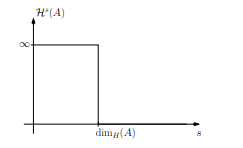
\includegraphics{dimension hausdorff.png}
\end{figure}
\begin{theo}\label{Hausdorff}
Soit $A \subset E. \exists !d \in \R_+\cup \{\infty\}$ tel que :
\begin{itemize}
\item $\mathcal{H}^s(A) = + \infty \quad \forall s<d$
\item $\mathcal{H}^s(A)=0 \quad \forall s>d$
\end{itemize}
Ce $d$ est unique et est appelé dimension de Hausdorff. La dimension d de Hausdorff est la valeur pour la quelle la fonction $s \mapsto \mathcal{H}^s(A)$ saute de la valeur $+ \infty$ à la valeur $0$. (voir figure \ref{schéma dimension hausdorff})

Donc
\begin{equation*}\label{x}
\begin{split}
d &= \inf \enstq{s \in [0, +\infty[}{\mathcal{H}^s(E)=0}\\
d &= \sup \enstq{t \in [0, +\infty[}{\mathcal{H}^t(E)=+\infty}
\end{split}
\end{equation*} 
La preuve de ce théorème repose sur le lemme suivant.
\end{theo}
\begin{rmq}
La dimension de Hausdorff de la frontière de l'ensemble de Mandelbrot vaut $2$. Ce résultat à été démontré en 1990 par Mitsuhiro \textsc{Shishikura}
\end {rmq}
\begin{lemme}\label{lemme}
$\textm{Soient} A \subset E \textm{et} 0\leq t <s<+\infty \textm{alors}$
\[\mathcal{H}^t(A) <+ \infty \Rightarrow \mathcal{H}^s (A)=0 \textm{et} \mathcal{H}^s(A)>0 \Rightarrow \mathcal{H}^t(A) = + \infty\]
\end{lemme}

\begin{proof}
$\textm{Soit} \epsilon > 0, A \subset E. \textm{on a :}$
\begin{equation*}\label{xx}
\begin{split}
\mathcal{H}^s_\epsilon (A)& \leq \inf_{\mathcal{D \in \mathcal{R}_\epsilon} (A)} \sum_{X \in \mathcal{D}} \epsilon ^{s-t} (diam X)^t \\
& = \epsilon^{s-t} \inf_{\mathcal{D \in \mathcal{R}_\epsilon} (A)} \sum_{X \in \mathcal{D}} (diam X)^t \\
& = \epsilon^{s-t} \mathcal{H}^t_\epsilon (A)
\end{split}
\end{equation*}
$\textm{En faisant tendre} \epsilon\rightarrow 0,$
\[\mathcal{H}^s (A) \leq \epsilon ^{s-t} H^t (A)\]
Donc \[\mathcal{H}^s _{\epsilon} (A) \rightarrow 0 \textm{lorsque} \epsilon \rightarrow 0\]
\end{proof}

\begin{proof}[Démonstration du théorème \ref{Hausdorff}]
$\textm{Soit} d' = \inf (s \geq 0, \mathcal{H}^s _\epsilon (A) < + \infty)$
Par définition, si $s<d \Rightarrow \mathcal{H}^s (A) = +\infty \textm {(voir théorème \ref{Hausdorff})}$
par le lemme \ref{lemme}, $\mathcal{H}^s(A)=0$ et il est clair que ce $d$ est unique.
\end{proof}

\begin{proposition}
$\exists c_{1} \textm{et} c_{2} | c_{1}N'_{\epsilon}\leq N_{\epsilon}\leq c_{2}N'_{\epsilon} $
\end{proposition}
\begin{proof}
Soit $C$ une courbe. 
Soit $\epsilon>0$.
\[\A=\inf \enstq{B(i, \frac{\epsilon}{2})}{C\subset \bigcup_{icIcR2} B(i, \frac{\epsilon}{2})}\]
On note \[N_\epsilon =card(A)\]
Soit \[M_a (C)=lim_{\epsilon\rightarrow0}(N_\epsilon\epsilon^{a}), a\geq0 \textm{la mesure de Hausdorff} \]
On note: \[D_{H}(\mathcal{C})=inf_{IR+} \enstq{a}{Ma(\mathcal{C})=0}\]
Soit $\mathcal{Q}$ un quadrillage dont les cases, (notées $Q_{ij}, i,j e Z$) ont pour côté $\epsilon$.
Soit \[\mathcal{A'}= \enstq{Q_{ij}}{\mathcal{C}\subset \bigcup_{i,j e Z^{2}}Q_{ij}}\]
On note \[N'_{\epsilon}=card(\mathcal{A'})\]
Soit \[\mathcal{M}_{a}'(\mathcal{C})=lim_{\epsilon\rightarrow0}(N'_\epsilon\epsilon^{a})\]
On note: \[D_{H}'(\mathcal{C})=inf_{IR+} \enstq{a}{Ma'(\mathcal{C})=0}\]
On veut montrer que pour un $\mathcal{C}$ donné, \[D_{H}(\mathcal{C})=D_{H}'(\mathcal{C})
\textm{c'est à dire :}  \forall a \in IR+, \mathcal{M}_{a}(\mathcal{C})=0\Leftrightarrow \mathcal{M}_{a}'(\mathcal{C})\]
$\Longrightarrow$/ Prouvons maintenant que \[\mathcal{M}_{a}(\mathcal{C})=0 \Rightarrow \mathcal{M}_{a}'(\mathcal{C})
\textm{c'est à dire} \lim \limits_{\epsilon \rightarrow 0}(N_\epsilon\epsilon^{a})=0 \Rightarrow lim_{\epsilon\rightarrow0}(N'_\epsilon\epsilon^{a})=0\]
Or \[\exists>0 | N'_{\epsilon} \leq cN_{\epsilon} \Rightarrow lim_{\epsilon\rightarrow0}(N_\epsilon\epsilon^{a})=0 \Rightarrow lim_{\epsilon\rightarrow0}(N'_\epsilon\epsilon^{a})=0\]
Or, \[\forall\epsilon > 0, N'_{\epsilon} \leq 4N_{\epsilon}\]
\begin{figure}[h]
\centering
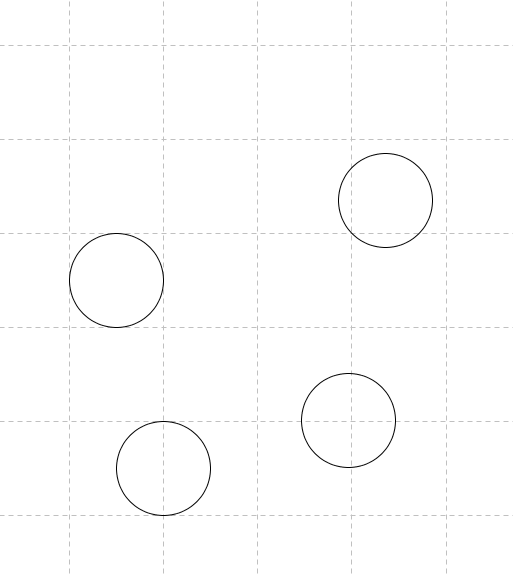
\includegraphics[width=10cm]{cases.png}
\caption{$\forall\epsilon > 0, N'_{\epsilon} \leq 4N_{\epsilon}$}
\label{fig:cases}
\end{figure}
Donc \[lim_{\epsilon\rightarrow0}(N'_\epsilon\epsilon^{a}) \leq lim_{\epsilon\rightarrow0}(4N_\epsilon\epsilon^{a})\]
c'est à dire\[lim_{\epsilon\rightarrow0}(N'_\epsilon\epsilon^{a}) \leq 4lim_{\epsilon\rightarrow0}(N_\epsilon\epsilon^{a})\]
c'est à dire \[lim_{\epsilon\rightarrow0}(N'_\epsilon\epsilon^{a}) \leq 0 \textm{(par hypothèse)}\] 
Or 
\begin{equation*}\label{y}
\begin{split}
N_\epsilon \geq 0 \textm{et} \epsilon \geq 0 & \Rightarrow 0 \leq \lim\limits_{\epsilon \Rightarrow 0} (N'_\epsilon\epsilon^{a}) \leq 0 \\
& \Rightarrow \lim\limits_{\epsilon \Rightarrow 0} (N'_\epsilon\epsilon^{a}) = 0 \textm{selon le théorème de l'encadrement}
\end{split}
\end{equation*}
Ainsi: \[\mathcal{M}_{a}(\mathcal{C})=0 \Rightarrow \mathcal{M}_{a}'(\mathcal{C})=0 \]
$\Longleftarrow$/ Montrons que \[\mathcal{M}_{a}(\mathcal{C})=0 \Leftarrow \mathcal{M}_{a}'(\mathcal{C})\]
\[\lim\limits{\epsilon\rightarrow0}(N_{\epsilon}\epsilon^{a})=0 \Leftarrow lim_{\epsilon\rightarrow0}(N'_{\epsilon}\epsilon^{a})=0\]
D'après la proposition \[\exists c' | N_{c\epsilon} \leq N\epsilon' \Rightarrow (lim_{\epsilon\rightarrow0}(N'_\epsilon\epsilon^{a})=0 \Rightarrow lim_{\epsilon\rightarrow0}(N_\epsilon\epsilon^{a})=0\]
Or \[N_{\sqrt[]{2}\epsilon} \leq N'_{\epsilon}\]
Ainsi \[\lim\limits{\epsilon\rightarrow0}(N_{\sqrt[]{2}\epsilon}(\sqrt[]{2}\epsilon)^{a}) \leq \sqrt[]{2}^{a}lim_{\epsilon\rightarrow0}N'_{\epsilon}\epsilon^{a}\]
Or \[N_{\sqrt[]{2}\epsilon} \geq 0 et (\sqrt[]{2}\epsilon)^{a} \geq0\]
On note \[\epsilon'=\sqrt[]{2}\epsilon\]
On voit que \[\epsilon'\rightarrow0 \Leftrightarrow \epsilon\Rightarrow0\]
Donc \[\lim\limits{\epsilon\rightarrow0}(N_{\epsilon}\epsilon^{a})=lim_{\epsilon\rightarrow0}(N'_{\epsilon}\epsilon'^{a})=0\]
Ainsi \[\mathcal{M}_{a}(\mathcal{C})=0 \Leftrightarrow \mathcal{M}_{a}'(\mathcal{C}) \]
Donc \[\inf_{IR+}{\enstq{a}{M'_{a}(\mathcal{C})=0}}= \inf_{IR+}{\enstq{a}{M_{a}(\mathcal{C})=0}}\]
Donc \[\mathcal{D}_{H}(\mathcal{C})=\mathcal{D}'_{H}(\mathcal{C})\]
\end{proof}

\end{document}
